% -*- Mode: latex; -*-
% $HeadURL: https://outreach.scidac.gov/svn/hpctoolkit/trunk/doc/manual/hpcviewer.tex $
% $Id: hpcviewer.tex 3336 2011-01-03 23:29:25Z tallent $


% ----------------------------------------------------------
% traceviewer
% ----------------------------------------------------------

\newcommand{\traceview}{Trace view}
\newcommand{\depthview}{Depth view}
\newcommand{\miniview}{Mini map view}
\newcommand{\callview}{Call path view}


% ===========================================================================
% ===========================================================================



\HPCToolkit{} provides the \hpctraceviewer{}~\cite{Tallent-MC-etal:2011:hpctoolkit-scalable-tracing} performance presentation tool for interactive examination of performance-trace databases.
\hpctraceviewer{} interactively presents a large-scale trace without concern for the scale of parallelism it represents.


% ===========================================================================
% ===========================================================================

\section{Launching}

\hpctraceviewer{} can either be launched from a command line (Linux/Unix platform) or by clicking the \hpctraceviewer{} icon (for Windows, Mac OS X and Linux/Unix platform).
The command line syntax is as follows:
\begin{quote}
\begin{verbatim}
  hpctraceviewer [options] [<hpctoolkit-database>]
\end{verbatim}
\end{quote}
Here, \texttt{<hpctoolkit-database>} is an optional argument to load a database automatically.
Without this argument, \hpctraceviewer{} will prompt for the location of a database.

The possible options are as follows:
\begin{itemize}

 \item \texttt{-consolelog}: Send log entries to a console in addition to a log file.
   (To get a console window, be sure to use java as the VM instead of javaw.)

 \item \texttt{-debug}: Log additional information about plug-in dependency problems.
\end{itemize}


% ===========================================================================
% ===========================================================================

\section{Views}

\begin{figure}[t]
\centering{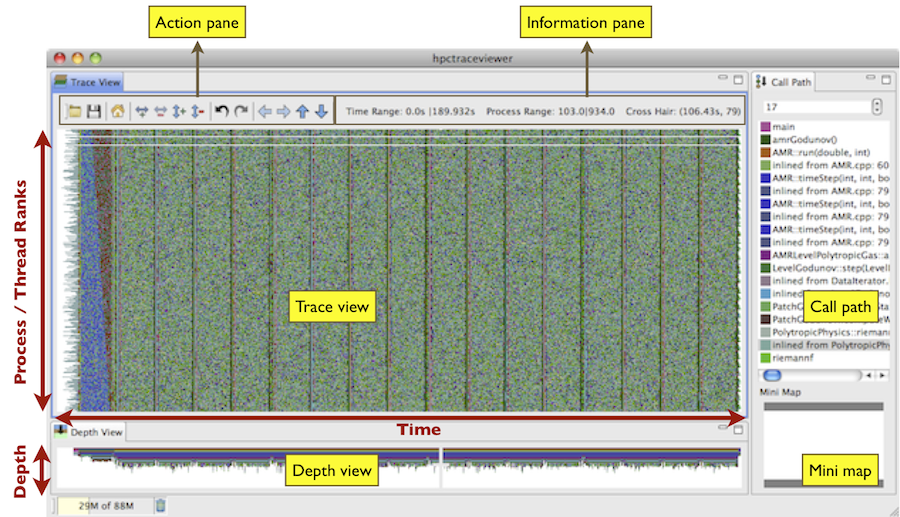
\includegraphics[width=\textwidth]{fig/hpctraceviewer-legend.png}}
\caption{An annotated screenshot of \hpctraceviewer{}'s interface.}
\label{fig:hpctraceviewer-legend}
\end{figure}

Figure~\ref{fig:hpctraceviewer-legend} shows an annotated screenshot of \hpctraceviewer{}'s user interface presenting a call path profile.
The annotations highlight \hpctraceviewer{}'s four principal window panes: \traceview, \depthview, \callview{} and \miniview.

\begin{itemize}
\item \textbf{\traceview} (left, top):
  This is \hpctraceviewer{}'s primary view.
  This view, which is similar to a conventional process/time (or space/time) view, shows time on the horizontal axis and process (or thread) rank on the vertical axis; time moves from left to right.
  Compared to typical process/time views, there is one key difference.
  To show call path hierarchy, the view is actually a user-controllable slice of the process/time/call-path space.
  Given a call path depth, the view shows the color of the currently active procedure at a given time and process rank.
  (If the requested depth is deeper than a particular call path, then \hpctraceviewer{} simply displays the deepest procedure frame and, space permitting, overlays an annotation indicating the fact that this frame represents a shallower depth.)

  \hpctraceviewer{} assigns colors to procedures based on (static) source code procedures.
  Although the color assignment is currently random, it is consistent across the different views.
  Thus, the same color within the Trace and Depth Views refers to the same procedure.

  The Trace View has a white crosshair that represents a selected point in time and process space.
  For this selected point, the Call Path View shows the corresponding call path.
  The Depth View shows the selected process.

\item \textbf{\depthview} (left, bottom):
  This is a call-path/time view for the process rank selected by the \traceview's crosshair.
  Given a process rank, the view shows for each virtual time along the horizontal axis a stylized call path along the vertical axis, where `main' is at the top and leaves (samples) are at the bottom.
  In other words, this view shows for the whole time range, in qualitative fashion, what the Call Path View shows for a selected point.
  The horizontal time axis is exactly aligned with the Trace View's time axis; and the colors are consistent across both views.
  This view has its own crosshair that corresponds to the currently selected time and call path depth.

\item \textbf{\callview} (right, top):
  This view shows two things: (1) the current call path depth that defines the hierarchical slice shown in the Trace View; and (2) the actual call path for the point selected by the Trace View's crosshair.
  (To easily coordinate the call path depth value with the call path, the Call Path View currently suppresses details such as loop structure and call sites; we may use indentation or other techniques to display this in the future.)

\item \textbf{\miniview} (right, bottom):
  The Mini Map shows, relative to the process/time dimensions, the portion of the execution shown by the Trace View.
  The Mini Map enables one to zoom and to move from one close-up to another quickly.

\end{itemize}

% ===========================================================================
% ===========================================================================

\section{\traceview}
\label{sec:hpcviewer:panes}

\traceview{} is divided into two parts: the top part which contains \emph{action pane} and the \emph{information pane}, and the main view which displays the traces. 

\begin{itemize}

\item \textbf{Open a view configuration} 
\includegraphics[scale=.5]{fig/hpctraceviewer-button-open.png}: Loading a saved view configuration. 
A view configuration file contains the information of the current range of time and process, as well as the depth and the position of the cross hair. 
\item \textbf{Save a view configuration} 
\includegraphics[scale=.5]{fig/hpctraceviewer-button-save.png}: Saving the current view configuration into a file. 
It is recommended to store the view configuration file in the same directory as the database. 
A view configuration file does not store the corresponding database, so it is possible to open 
\item \textbf{Home} 
\includegraphics[scale=.5]{fig/hpctraceviewer-button-home-screen.png}: Resetting the view configuration into the original view, i.e., viewing traces for all times and processes.

\item \textbf{Horiontal zoom-in} 
\includegraphics{fig/hpctraceviewer-button-zoom-in-time.png}: Zooming-in the time range of the traces.
\item \textbf{Horiontal zoom-out} 
\includegraphics{fig/hpctraceviewer-button-zoom-out-time.png}: Zooming-out the time range of the traces.
\item \textbf{Vertical zoom-in} 
\includegraphics[scale=.5]{fig/hpctraceviewer-button-zoom-in-process.png}: Zooming-in the process range of the traces.
\item \textbf{Vertical zoom-out} 
\includegraphics[scale=.5]{fig/hpctraceviewer-button-zoom-out-process.png}: Zooming-out the process range of the traces.
\item \textbf{Undo} 
\includegraphics[scale=.5]{fig/hpctraceviewer-button-undo.png}: Canceling the action of zoom or navigation and returning back to the previous view configuration.
\item \textbf{Redo} 
\includegraphics[scale=.5]{fig/hpctraceviewer-button-redo.png}: Redoing of previously undo change of view configuration.
\item \textbf{Navigation buttons} 
\includegraphics[scale=.5]{fig/hpctraceviewer-button-go-east.png}, 
\includegraphics[scale=.5]{fig/hpctraceviewer-button-go-west.png}, 
\includegraphics[scale=.5]{fig/hpctraceviewer-button-go-north.png}, 
\includegraphics[scale=.5]{fig/hpctraceviewer-button-go-south.png}: Navigating the trace view to the left, right, up and bottom, respectively. It is also possible to navigate with the arrow keys in the keyboard. Since the \traceview{} does not support scrool bars, the only way to navigate is through navigation buttons (or arrow keys).


\end{itemize}

% ===========================================================================
% ===========================================================================

\section{Limitations}

Some important \hpctraceviewer{} limitations are listed below:
\begin{itemize}

\item \textbf{No image save or print}.
	At the moment \hpctraceviewer{} does not support saving and printing images of the traces.


\end{itemize}
